\documentclass{beamer}
\usepackage{amsmath}
\usepackage{color}
\usepackage{ulb}
\title{Implementation of Decision Tree Classifiers\\
ID3 versus C4.5}
\author{Depuydt Antoine\\ Dansy Efila \\Mudura Mircea}

\date{May, 2017}
\begin{document}
\maketitle

\addtobeamertemplate{navigation symbols}{}{%
    \usebeamerfont{footline}%
    \usebeamercolor[fg]{footline}%
    \hspace{1em}%
    \insertframenumber/\inserttotalframenumber
}

\section{Introduction}
\begin{frame}
\frametitle{Introduction}
\begin{itemize}
\item Data mining: compress, understand and predict
	\vfill
	\begin{itemize}
		\item Clustering
		\vfill
		\item Classification
		\vfill
		\item Regression
		\vfill
		\item ...
	\end{itemize}
\vfill
\item Techniques to find links
	\vfill
	\begin{itemize}
		\item Linear Regression
		\vfill
		\item Decision Trees
		\vfill
		\item Neural Networks
		\vfill
		\item ...
	\end{itemize}
\end{itemize}
\end{frame}


\begin{frame}
\frametitle{Classification}
	\begin{itemize}
		\item Classical example: play tennis today?
		\vfill
		\begin{itemize}
			\item \textbf{Features}:
			\begin{itemize}
				\item Outlook: sunny, overcast, rainy
				\vfill
				\item Temperature: hot, cool, cold
				\vfill
				\item Wind: high, weak
				\vfill
				\item Humidity: high, normal
			\end{itemize}
			\vfill
			\item \textbf{Class labels}:
				\begin{itemize}
				\item Yes
				\vfill
				\item No
				\end{itemize}			

		\end{itemize}
	\end{itemize}
\end{frame}

\begin{frame}
\frametitle{Decision Tree}
	\begin{itemize}
		\item Visual model, easily understandable
		\vfill
		\item Model: tree with \color{blue}decision \color{black}and \color{green}leaf nodes \color{black}
	\end{itemize}
	\begin{center}
		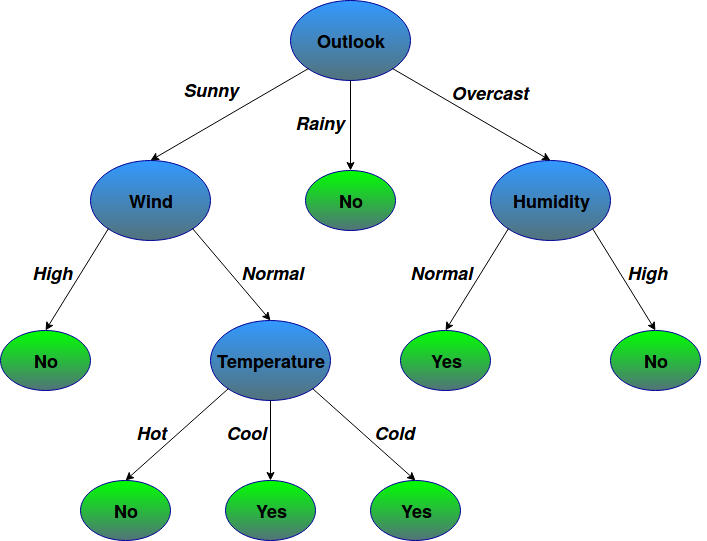
\includegraphics[scale=0.35]{Images/DecisionTree.png}
	\end{center}

\end{frame}

\begin{frame}
\frametitle{Premise}
\begin{itemize}
\item Given a training data-set 
\vfill
\item Recursively split on a node:
\vfill
\item If node is pure return leaf (class value)
\vfill
\item Else compute entropy \& info gain:
\begin{itemize}
\vfill
\item Shannon's entropy: $E(S)= \sum_{i}{} - p_i log_2(p_i) $
\vfill
\item Subtree gain: $Gain(T,X)=E(T)-E(T,X)$
\vfill
\end{itemize}
\end{itemize}
\end{frame}


\begin{frame}
\frametitle{ID3 versus C4.5}
	\begin{itemize}
		\item Goal: implement ID3 and C4.5 algorithms
		\vfill
		\item Objectives: compare ID3 and C4.5 output
		\vfill
		\begin{itemize}
			\item Compare ID3 and C4.5
			\vfill
			\item Create an application that classifies any data using both algorithms
		\end{itemize}

	\end{itemize}

\end{frame}

\begin{frame}
\frametitle{ID3}
\begin{itemize}
\item Initial implementation of decision trees
\item Top down approach
\item Split current node based on information gain:

\end{itemize}

\end{frame}

\begin{frame}
\frametitle{C4.5}

\end{frame}

\begin{frame}
\frametitle{K-fold cross validation}

\end{frame}

\begin{frame}
\frametitle{Demonstration}

\end{frame}

\end{document}